Due to the very different comprehension of certain terms by different people from different fields of research 
The first part of my work during the internship was the creation of a glossary describing certain given terms
... in order to unify the understanding of these terms and create a basis for discussions ans researches.

- The glossary was later taken as standard for this tasks ...
- and deals with the terms: \emph{service}, \emph{system}, \emph{system of systems}, \emph{architecture}, \emph{service-oriented architecture}, \emph{configuration}, \emph{static reconfiguration}, \emph{dynamic reconfiguration}, \emph{inter-core communication}, \emph{intra-core communication} and \emph{binding}.
The most important parts of this glossary will be covered within this chapter.
- furthermore a database with the used literature was created in order to provide the necessary references for the glossary and provide a ... where to find further information for the employees. 

- disambiguity safety and security
- what is safety and fault tolerance

\section{Related instances}
\subsection{ISO 262662 international standard}
\subsection{MISRA}
\subsection{AUTOSAR}
\section{service}




\section{System}

\label{ch:system}
This chapter explores various definitions of the term system, as well as related hierarchies and terminology. Because of its reappearance in later chapters, the term \emph{embedded system} is also covered.

\subsection{Definitions}
Definition of \emph{system}\index{system} by different sources:
\begin{description}
\item [ISO/IEC 15288] .
The ISO/IEC 15288\footnote{The ISO/IEC 15288 standard is a \emph{System Engineering Standard} and defines processes and terminology for systems created by humans \cite{ISO_15288}.} standard states that systems \textit{``are man-made and may be configured with one or more of the following: hardware, software, data, humans, processes (e.g. processes for providing services to users), procedures (e.g. operator instructions), facilities, materials and naturally occurring entities''} \cite{ISO_15288}.

\item [GENESYS architecture].
Definition of system according to Obermaisser and Kopetz: \emph{``an entity that is capable of interacting with its environment and is sensitive to the progression of time''} \cite[p.7]{genesys}.
The \emph{environment}\index{environment} is a system itself, which produces input for other systems and acts according to their outputs. Which elements (cf. section \ref{sec:system_element}) belong to the system, and which to the environment, is a matter of perspective. 

\item [ISO 26262].
The ISO 26262 standard defines a system as a \emph{``set of elements that relates at least a sensor, a controller and an actuator with one another''} \cite{iso26262:1}. This definitions is already a bit more specific with a focus on the automotive industry.

\item [ARROWHEAD].
Arrowhead has a bit slightly different notion of the concept \emph{system}. With respect to their view, a system is simply an artifact which provides and/or consumes \emph{services} (cf. chapter \ref{ch:service}) \cite{arrowhead_inpr}, what implies that systems are directly related to service oriented architectures (cf. chapter \ref{ch:soa}).

\item [AUTOSAR].
\begin{quote}
\emph{``An integrated composite that consists of one or more of the processes, hardware, software, facilities and people, that provides a capability to satisfy a stated need or objective''} \cite{autosar_glossary}.
\end{quote}

There is no indication that system have any internal structure, or that services are exchanged inside of them, which is the case according to the other sources. In this definition the is more like a component (cf. \emph{``It may also be referred to as Component or Device''} \cite{arrowhead_inpr}).
\end{description}

The sources may differ a bit in terms of specificity, but all in all, there are no critical contradictions or discordances. 

Throughout this glossary the naming convention of the ISO 26262 standard, which can be seen in figure \ref{fig:26262_disambiguation} is used.


\subsubsection{System Element}
\label{sec:system_element}
\begin{quote}
\emph{``element - system or part of system including components hardware, software, hardware parts, and software units''}, \cite{iso26262:1}
\end{quote}
This definition of \emph{element}\index{system!system element} is taken from the ISO 26262 standard. It is a very generic term and thus it is not advisable to define it for any entities at a specific layer or with a specific characteristic. Instead, according to the quote, it can be more or less any entity of a system, since a system itself is defined as ``set of elements'' \cite{iso26262:1}.

\begin{figure}[ht]
\centering
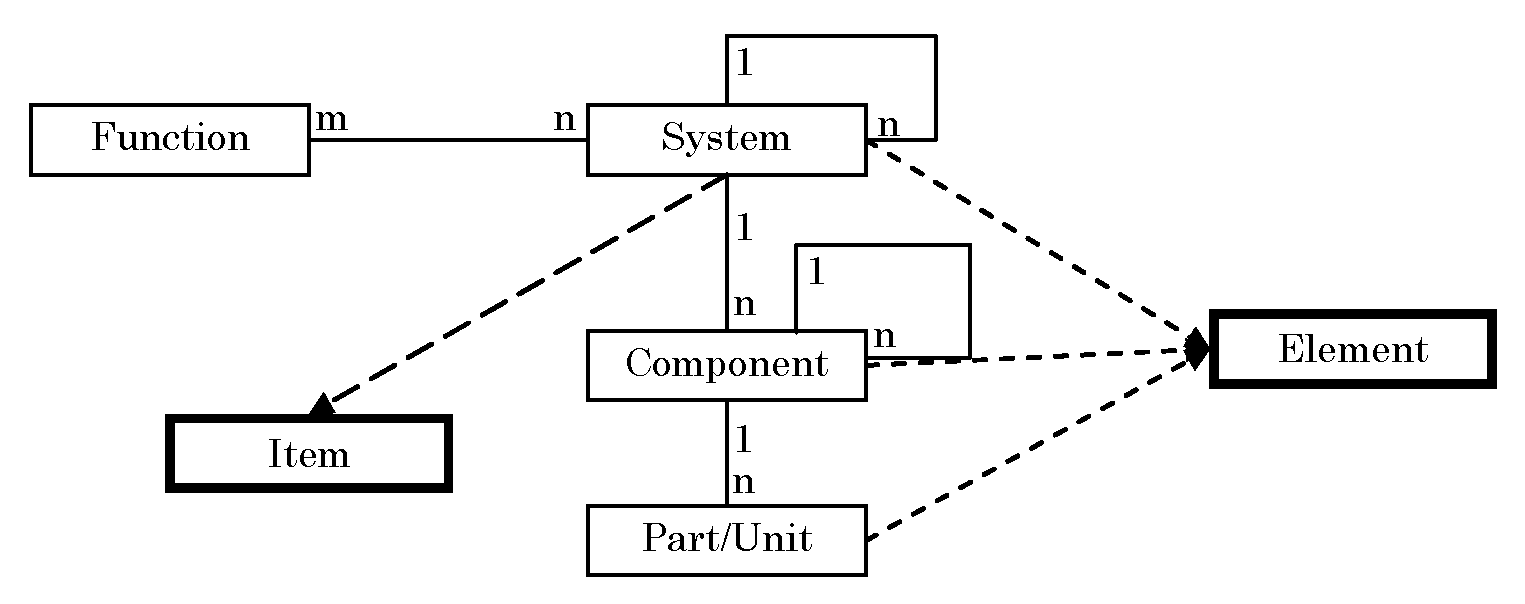
\includegraphics[scale=0.5]{26262_disambiguation_system_etc.pdf}

\caption{Relation of \emph{system}, \emph{component} and \emph{element} according to ISO 26262 \cite{iso26262:course1}.}
\label{fig:26262_disambiguation}
\end{figure}

\subsection{Definition for the EMC2 project}
The most crucial aspects are combined and emphasised in the following definition.

\begin{myquote}
A system is a hierarchical composed, time sensitive element, which interacts with the environment by processing input and providing output in turn.

It is concerned with satisfying a specific need or purpose and disposes of a, more or less complex, internal structure, which may include hardware, software and data.
\end{myquote}

As stated, the time domain has to be taken into account to describe the behaviour of a system. Thus, a time model is required. Distributed systems usually deploy physical clocks for splitting the time in equally spaced intervals \cite[p.7-8]{genesys}.

For the scope of this paper, the overall system is defined as a \textbf{vehicle} in order to be able to provide some examples. The environment consists therefore of other vehicles or the surrounding infrastructure. Nevertheless, the entire traffic could also be taken as a system and the environment would then be a different one; for example entities like roads, weather conditions and the like.

\subsection{System of Systems}
Systems are hierarchical and can be composed or decomposed into sets of interacting constituting systems. Often this is referred to by the term \emph{System of Systems (SoS)}\index{system of systems} \cite[p.7]{genesys}. Thus, the SoS is in general the level above a given system and is therefore dependent on the definition of the related systems. With respect to our previous example of a system vehicle, a SoS could be for example the traffic of Graz, with many vehicles participating.

This is in accordance with the definition of system by Arrowhead: \emph{``collaborating, compliant systems become system-of-systems and SoSs can be parts of other, bigger SoSs in turn''} \cite{arrowhead_inpr}. 

System of systems features the following five characteristics:
\begin{itemize}
\item operational independence of its systems,
\item management independence of the systems,
\item evolutionary development,
\item emergent behaviour, and
\item geographic distribution \cite{arrowhead_inpr}.
\end{itemize}
Concerning this definition, it has to be stated that \emph{geographic distribution} it not necessarily always the case when operating with embedded systems.


\subsection{System Layers}
\label{ch:system_layers}
The parts of a system can be divided into different layers of implementation, for this kind of abstraction makes it easier for human beings to comprehend the overall relations. Unfortunately each field of research features its own way of fractionising systems and most of the approaches are hardly hardly compatible or even contradicting. The following, a segmentation from the GENESYS architecture\index{architecture!GENESYS architecture}, revealing a quite hardware and embedded systems oriented point of view, and a more abstract view from the ARROWHEAD project, are investigated in more detail.

\subsubsection{System Layers by GENESYS}
The GENESYS architecture by Obermaisser and Kopetz distinguish between three different layers, denoted \emph{chip-level}, \emph{device-level} and \emph{system-level} \cite[p.44]{genesys}. An example of the hardware elements at different levels by means of a system vehicle can be seen in figure \ref{fig:integration_levels}.
\begin{description}
\item [System Level] .
The system level consists of \emph{Devices}, which are themselves logically self-contained apparatus. With respect to a system vehicle this could be for example an ECU, a sensor, an actuator or the like \cite[p.45]{genesys}.
\item [Device Level] .
The devices at the system level, contain a certain internal structures themselves. In case of embedded systems these are in most cases \emph{Chips} \cite[p.45]{genesys}, like the the AURIX\textsuperscript{TM} \footnote{The AURIX (Automotive Realtime Integrated NeXt Generation Architecture) is a new family if multi core microcontroller, adjusted to the needs of the automotive industry - \url{http://www.infineon.com/cms/en/product/microcontroller/32-bit-tricore-tm-microcontroller/aurix-tm-family/channel.html?channel=db3a30433727a44301372b2eefbb48d9}} chip, which is frequently used in the automotive industry.
\item [Chip Level] .
According to the implementation layers in the GENESYS architecture, the chip level is the lowest level of implementation. In case of an MPSoC (Multiprocessor System-on-Chip)\footnote{A \emph{Multiprocessor System-on-Chip} is an integrated circuit which uses multiple processors and is often used for embedded applications \cite{wiki_MPSoC}.} this level contains the single IP Cores of the chip \cite[p.46]{genesys}
\end{description}

\begin{figure}[ht]
\centering
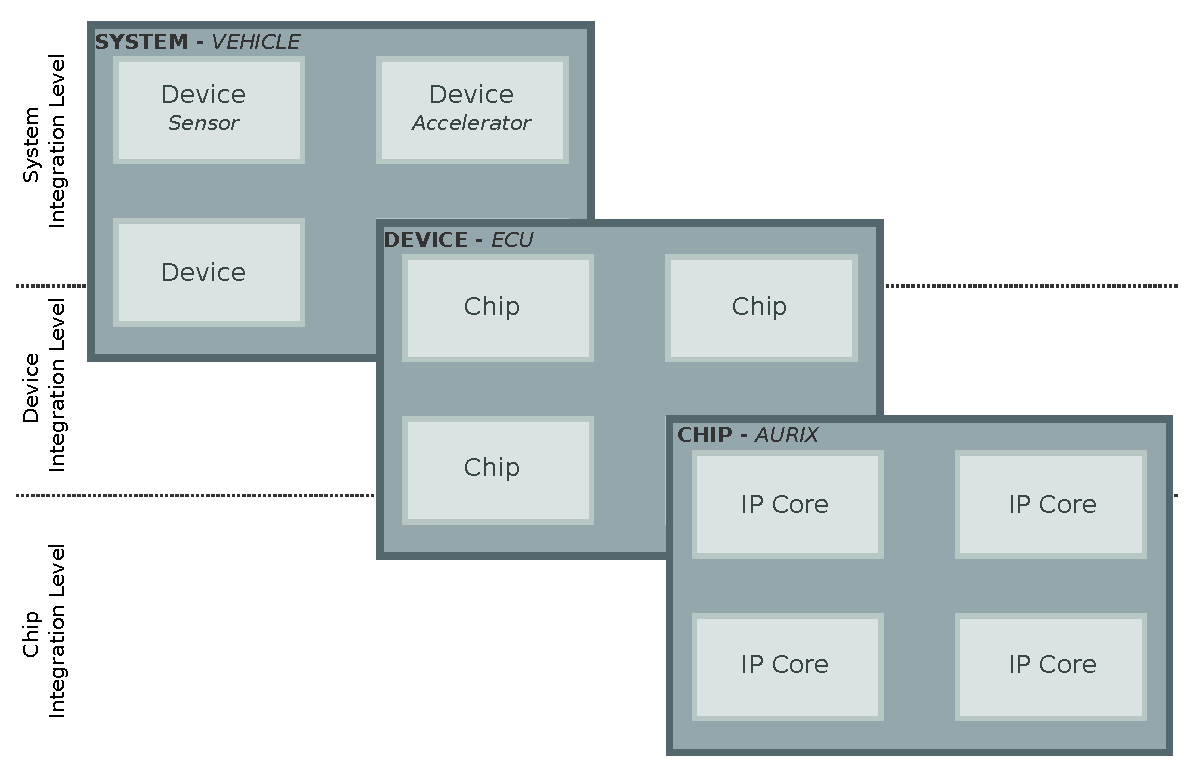
\includegraphics[width=\textwidth]{system_levels.pdf}
\caption{The hierarchy of the integration levels of the system ``vehicle'' with examples}
\label{fig:integration_levels}
\end{figure}

\subsubsection{System Layers by ARROWHEAD}

The Arrowhead Framework provides an hierarchy by means of documentation documents, which are spitted in the three levels \emph{system-of-systems}, \emph{system} and \emph{service} \cite{arrowhead_inpr}. Their involved documents and relations are pictured in figure \ref{fig:sys-arrowhead}.

\begin{description}
\item [System-of-systems]. The levels features the two documents \emph{SoS Description (SoSD)}\index{system of systems!SoS description} and \emph{SoS Design Description (SoSDD)}\index{system of systems!SoS Design Description}. The differ in the amount of information they are revealing. While the first represents only an abstract view, the second also reveals the implementation of the SoS and its technologies \cite{arrowhead_inpr}.
\item [System]. The system level comes with the two documents \emph{System Description (SysD)}\index{system!system description} and \emph{System Design Description (SysDD)}\index{system!system design description}. Just as at the SoS level the first one features a kind of black box opacity and the second a white box view (cf. section \ref{sec:blacknwhite}) \cite{arrowhead_inpr}.
\item [Service]. The service level contains the four documents \emph{Service Description (SD)}\index{service!service description}, \emph{Interface Design Description (IDD)}\index{interface!interface design description}, \emph{Communication Profile (CP)}\index{communication!communication profile} and \emph{Semantic Profile (SP)}\index{semantic profile}. The service description is referred to in \ref{sec:service_structure}.
\end{description}

\begin{figure}[ht]
\centering
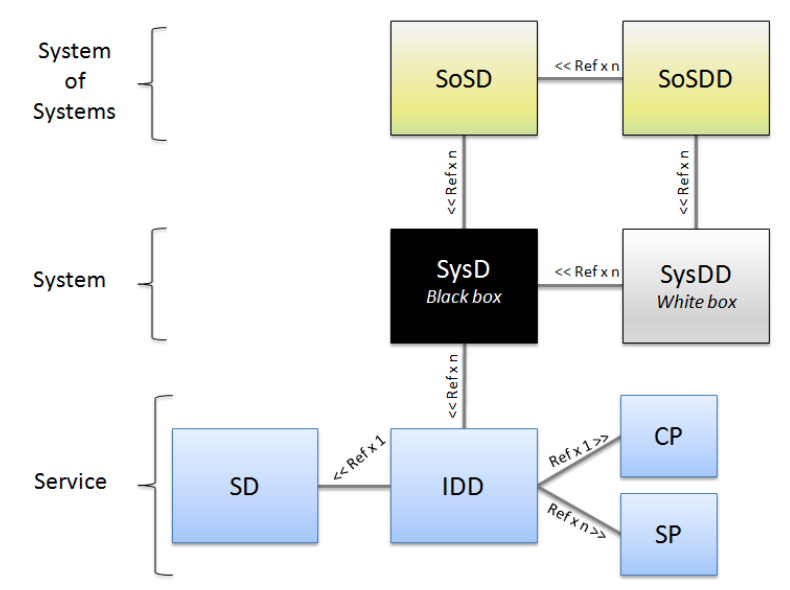
\includegraphics[scale=0.4]{arrowhead-documentation-relationship.png}
\caption{Relation of System, SoS and Service to one another \cite{arrowhead:presentation}.}
\label{fig:sys-arrowhead}
\end{figure}

All the documents exist as templates which should be filled out during the development process of a system. They feature a XML like style in order to be human and machine readable at the same time.

Developed systems can then be constituted to SoS by an underlying cloud, as depicted in figure \ref{fig:arrowhead-framework}. All the system have specified and standardised interfaces and work together by means of three \emph{core services}\index{service!core service}, labeled II, AI and SM.
\begin{description}
\item [Information Assurance\index{information assurance} (IA)] .
This service is responsible for providing secure information exchange through authorization and authentication \cite{arrowhead:presentation}.
\item [Information Infrastructure\index{information infrastructure} (II)] .
The II service enables the listing of the services in the \emph{service repository}\index{service!service repository} (cf. section \ref{sec:structure_of_soa}) and their discoverability \cite{arrowhead:presentation}.
\item [System Management\index{system!system management} (SM)] .
This is the core service for the system of systems composition and features logging and monitoring abilities \cite{arrowhead:presentation}.
\end{description}

\begin{figure}[ht]
\centering
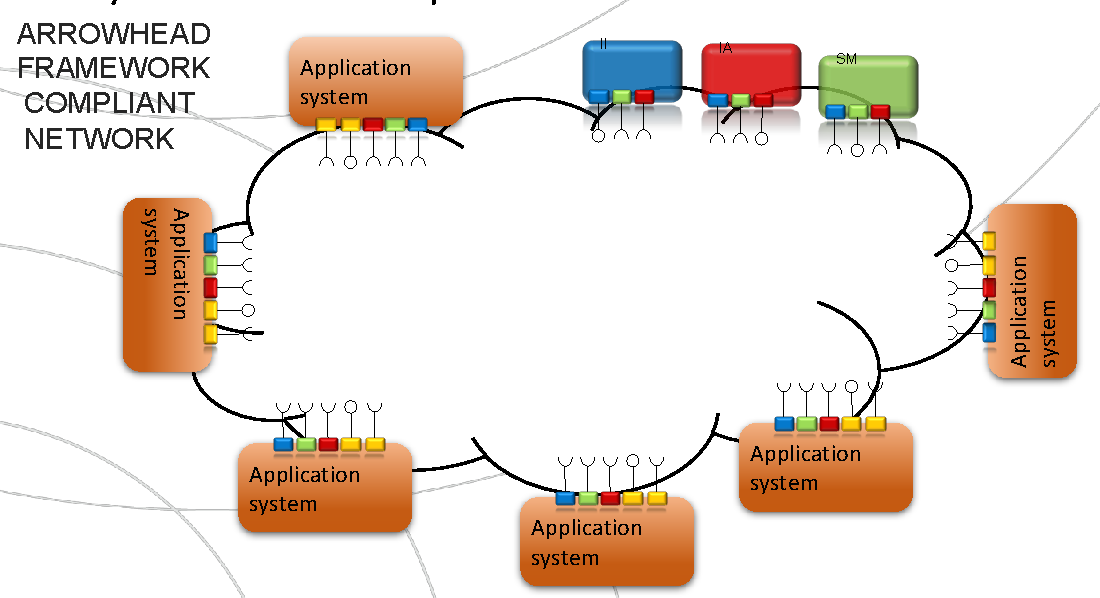
\includegraphics[scale=0.8]{arrowhead-framework.pdf}
\caption{Implementation example of an ARROWHEAD framework \cite{arrowhead:presentation}.}
\label{fig:arrowhead-framework}
\end{figure}

\subsection{Embedded System}
\label{sec:embedded_system}

\emph{Embedded systems}\index{system!embedded system} are computational modules integrated to physical devices and equipment. The have a predefined set of tasks and requirements and are capable of processing information \cite{rodrigues2011} \cite[p.xiii]{marwedel}. 

Compared to general-purpose computation systems they usually dispose of less processing resources and come with narrower operation ranges, but at the same time they feature a high efficiency by optimally managing the available resources \cite[p.283]{alippi} \cite[p.5]{marwedel}. Also, their presence is usually quite unobtrusive, because instead of mice and keyboard the user interface consists of typical input devices like buttons, steering wheel, or pedals.

Embedded systems are \emph{reactive systems}\index{system!reactive system}, what means that they perform a continuous interaction with the environment. The connection to the physical environment is realised by means of sensors, responsible for collecting information, and actuators for performing the actual reaction \cite[p.8-9]{marwedel}. 

During operation, embedded systems are in a certain state, waiting for input. When provided with that, they perform computations and generate an output, which is handed back to the environment \cite[p.9]{marwedel}.

Embedded systems in safety-critical applications have to care about the issues \emph{time constraints}, \emph{dependability} and \emph{efficiency requirements}.

\begin{description}
	\item [Time constraints].
	One challenge of Embedded Systems is the meeting of so called \emph{time constraints}\index{time constraint}, which basically means the conduction of a computation within a specified time \cite[p.8-9]{marwedel} \cite{rodrigues2011}. Kopetz states \emph{``A time-constraint is called hard if not meeting that constraint could result in a catastrophe''} \cite{kopetz}.
	\item [Dependability].
	Embedded systems, operating in safety-critical environment, like nuclear power plants, cars, trains or aircraft, must be \emph{dependable}\index{dependability}, for they are directly connected to the environment and have immediate impact on it. The Dependability is split up in further aspects - in detail \emph{Reliability} (cf. section \ref{sec:reliability}), \emph{Maintainability}, \emph{Availability} (cf. section \ref{sec:availability}), \emph{Safety} (cf. chapter \ref{ch:functional_safety}) and \emph{Security} \cite[p.4-5]{marwedel}.
	\item [Efficiency requirements\index{efficiency requirements}].
	Efficiency is a key concept of embedded systems and is concerned with providing a maximum computation performance while minimizing the required energy. The efficiency is measured in ``operations per Joule'' and has been been increasing almost exponentially during the last twenty years.
\end{description}






\section{Component}

\label{ch:component}

For the EMC2 project it is crucial to achieve a clear distinction between the term \emph{component}\index{component} and \emph{service}\index{service} (cf. chapter \ref{ch:service}). Due to the historic development of \emph{service oriented architecture} (cf. chapter \ref{ch:soa}), as successor of the \emph{component based software engineering} (cf. chapter \ref{ch:cbse}), those terms have often been put on a level, giving rise to confusion. 

Another issue is the term \emph{software component}\index{component!software component}, which leads to the question, whether components are pure software elements.

In the following some definitions from different relevant resources are presented and discussed, with the aim to eliminate those ambiguities. The relation of component to service is investigated in section \ref{sec:relation_service_component}, subsequent to the definition of service.

\subsection{Definitions}

\begin{description}
	\item [GENESYS reference architecture] .
	Obermaisser and Kopetz state that a component is a software or hardware unit that performs a specified computation within a given period of time \cite[p.38]{genesys} and communicates with other components by means of specific \emph{interfaces} (cf. section \ref{sec:component_interfaces}). Like systems, components are hierarchical and therefore dependent on the point of view - from a different viewpoint a quantity of components may be seen as a single component. With respect to this definition all entities in figure \ref{fig:integration_levels} (\emph{System}, \emph{Sensor}, \emph{AURIX}, etc.) can be denoted as components.

	\item [ISO26262] .
	The ISO 26262 standard supports this concept by its definition of a component as a \emph{``non-system level element that is logically and technically separable and is comprised of more than one hardware part or one or more software units''} \cite{iso26262:1}.
\end{description}


\subsubsection{Software Component}
The following sources refer explicitly to \emph{software components}.

\begin{description}
	\item [Szyperski].
	Szyperski features a definition with emphasis on the software oriented point of view: \emph{``Software components are binary units of independent production, acquisition, and deployment that interact to form a functioning system''} \cite[p.xxi]{szyperski}.

	\item [AUTOSAR].
	\begin{quote}
	\emph{``Software-Components are architectural elements that provide and/or require interfaces and are connected to each other through the Virtual Function Bus to fulfill architectural responsibilities''} \cite{autosar_glossary}.
	\end{quote}

	AUTOSAR defines a \emph{Software Component} as encapsulation for parts of the automotive functionality, but it dictates no specific ``granularity'', meaning that an AUTOSAR software component might be either a \emph{``a small, reusable piece of functionality (such as a filter) or a larger block encapsulating an entire sybsystem. \cite{autosar}''}
	
	\item [Software Engineering Institute].
	In software engineering a component is usually considered as a piece of software with specific functionality. The \emph{Software Engineering Institute\footnote{\emph{``The Software Engineering Institute (SEI) is a non-for-profit Federally Funded Research and Development Center (FFRDC) at Carnegie Mellon University, specifically established by the U.S. Department of Defense (DoD) to focus on software and cybersecurity.''} - \url{http://www.sei.cmu.edu/about/organisation/index.cfm}}} describes a component by means of another definition by Szyperski:
	\begin{quote}
	\emph{``A software component is a unit of composition with contractually specified interfaces and explicit context dependencies only. A software component can be deployed independently and is subject to composition by third parties''} \cite{szyperski}.
	\end{quote}

	\item [ARCITURA]\footnote{Arcitura\textsuperscript{TM} Education Inc. is a global provider of progressive, vendor-neutral training and certification programs. It is also the owner of \url{http://www.serviceorientation.com} \cite{arcitura}, which served as valuable sources and is also the located of the related citation - \url{http://arcitura.com/about}}.
	\emph{``A component is a unit of logic that exists as a standalone software program as part of a distributed computing architecture''} \cite{arcitura}.
 \end{description}


\subsubsection{Definition for the EMC2 project}


\begin{myquote}
A component is a logical and technical separable hardware or software unit that is capable of performing a specific computation.

It offers an abstraction that simplifies the understanding of complex systems. Therefore they have to be hierarchical, meaning that components can be composed to other, larger, components.
\end{myquote}

As suggested by this definition the term component should be used for both, software hardware. If not denoted specifically as \emph{software component}\index{component!software component} or \emph{hardware component}\index{component!hardware component}, the term can be referred to both throughout this glossary.

A component can be seen as \emph{black box} (cf. chapter \ref{sec:blacknwhite}), meaning that the more or less complex internal structure is invisible or not of concern for the user. Therefore, other components stay unaffected from modifications of this internal structure, given that the behaviour at the \emph{Linking Interface} (cf. section \ref{sec:component_interfaces}) remains unaffected \cite[p.38-39]{genesys} \cite{autosar_intro} \cite{sametinger}.

As a self-contained subsystem, it can be developed and tested independently, and latter be used as building block for systems or higher level components. In other words, the components are the basic building blocks of a system \cite{ning}. 

Nevertheless, not everything is a component. According to Sametinger, an algorithm in a book is not a component, but it has to be implemented by means of an arbitrary programming language and equipped with well-defined interfaces in order to become a component \cite[p.2-3]{sametinger}.


\subsection{Component Interfaces}
\label{sec:component_interfaces}


The interfaces are necessary for any interaction with other components. In the following two different approaches for describing these interfaces are presented. The first one is from the \textbf{GENESYS project} and features a quite implementation oriented point of view. The second definition, by \textbf{AUTOSAR}, is more abstract and better adjusted to the service oriented architecture paradigm.



\subsubsection{Interfaces by GENESYS}
Following the definition from Obermaisser and Kopetz, each component may dispose of up to four interfaces for communication with other entities. The \emph{Linking Interface}, the \emph{Local Interfaces} and the \emph{Technology Independent-} or \emph{Technology Dependent Interface}. They are illustrated in figure \ref{fig:component_interfaces} \cite[p.40-41]{genesys}.

\begin{description}
\item [Linking Interface (LIF)\index{interface!linking interface}]. 
The \emph{Linking Interface} is a message based interface and responsible for offering the component's services. The LIF is dependent on the level of integration, e.g. Inter-IP Core LIF at chip level or Inter-Chip LIF at device level. Nevertheless, it is used only for communication to other components at the same layer and also the only place, where a component may provide its services to other components \cite[p.9]{genesys}.

The \emph{Linking Interfaces} are always technology agnostic, which means that they do not expose details on their implementation or \emph{Local Interfaces}. Accordingly, the implementation can be modified, without other components noticing, as long as the specification at the LIF remains unchanged \cite[p.9, 40-41]{genesys}.

\item [Local Interface\index{interface!local interface}]. 
The \emph{Local Interfaces} establish the connection between a component and its local environment, which could consist of sensors, actuators and the like. If the environment is modified, the semantics and timing of the data should stay the same in order to do not violate the specification. A \emph{Local Interface} could also be mapped to a \emph{LIF} of a component at the next-higher level - this is known \emph{gateway component} (cf. chapter \ref{ch:communication}) and enables different layers to communicate with each other.

Components do not necessarily require local interfaces. Such are denoted \emph{Closed Components}\index{component!closed component} \cite[p.40-41]{genesys}.

\item [Technology Independent Interface (TII)\index{interface!technology independent interface}].
The \emph{TII} is the instrument for configuring and reconfiguring a component, e.g. assigning a name, configuring input and output ports or monitoring the resource management. Starting, restarting and resetting the component is also executed through this interface. The TII communicates with the hardware, the operating system and the middleware, but not with the \emph{application software (service)}\index{application software}, which is reserved for the LIF \cite[p.40-41]{genesys}.

\item [Technology Dependent Interface (TDI)\index{interface!technology dependent interface}]. 
The \emph{Technology Dependent Interface} enables a look inside the component and allows to inspect internal variables and processes. Thus, it is reserved for people who bring a deep understanding of the components internals and is of no relevance for the user of the LIF services \cite[p.40-41]{genesys}. 
\end{description}

\begin{figure}[ht]
\centering
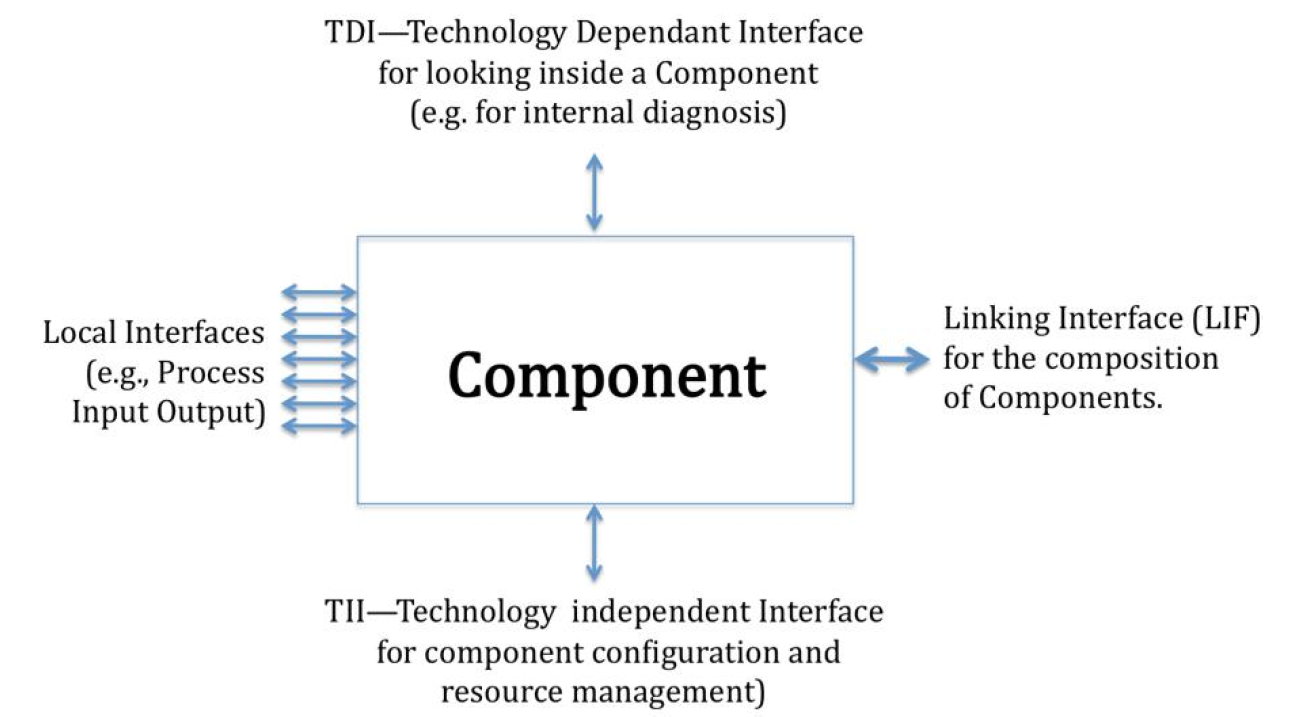
\includegraphics[scale=0.4]{component_interfaces.png}
\caption{The interfaces of a component, with respect to the \textbf{GENESYS architecture} \cite[p.40]{genesys}}
\label{fig:component_interfaces}
\end{figure}


\subsubsection{Interfaces by AUTOSAR}

AUOSAR follows a slightly more abstract approach concerning the interfaces of a component. According to their definition, a component may dispose of a number of \emph{ports}\index{port}. A port belongs to one component only and is the interface a component uses to communicate with other components.

Within this context, the term \emph{interface}\index{interface} specifies a kind of contract or specification, on which services can be called at this port, and the format of the data emitted at this port.

There are four different types of interfaces, belonging to the two different communication patterns \textbf{Client-Server} and \textbf{Sender-Receiver}: \cite{autosar_intro}

\begin{description}
\item [Client-Server Communication].
When this kind of communication is performed the \emph{client-component}\index{component!client component} requests the a specific service from the \emph{server-component}\index{component!server component} and sends necessary parameters. The server then processes the incoming request and returns a response. A single component can be a server and a client at the same time \cite{autosar_intro}. A schematic illustration of this type of communication is pictured in figure \ref{fig:autosar_client-server}, where SW-C denotes \emph{software component}\index{component!software component}.

\item [Sender-Receiver Communication].
The \emph{Sender-Receiver} approach is a bit different. The task of the sender is to distribute his information to one or more receivers, without ever getting a response in form of data or control flow. In fact he does not even know the number or identity of the receivers. Those have to decide on themselves, how to deal with the received data (cf. figure \ref{fig:autosar_sender-receiver}) \cite{autosar_intro}.
\end{description}

The different ports and their properties are visualized in figure \ref{fig:autosar_ports}. 

\begin{figure}[ht]
\centering
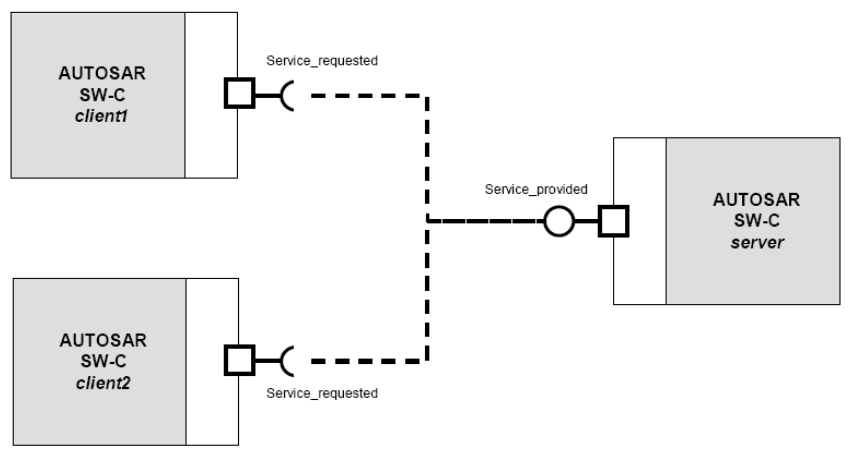
\includegraphics[scale=0.4]{autosar_client-server.png}
\caption{Illustration of the client-server communication \cite{autosar_intro}.}
\label{fig:autosar_client-server}
\end{figure}

\begin{figure}[ht]
\centering
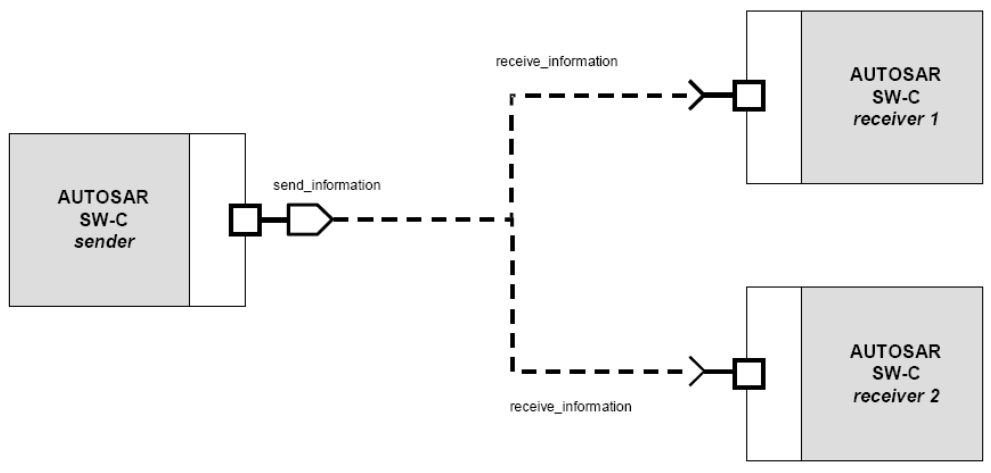
\includegraphics[scale=0.4]{autosar_sender-receiver.png}
\caption{Illustration of the sender-receiver communication \cite{autosar_intro}.}
\label{fig:autosar_sender-receiver}
\end{figure}

\begin{figure}[ht]
\centering
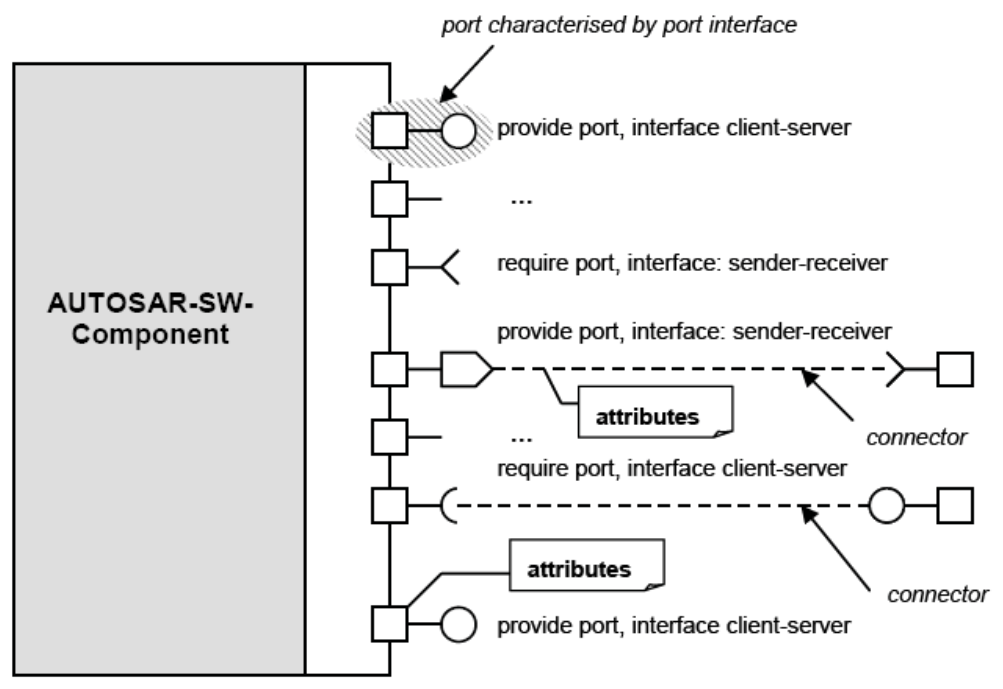
\includegraphics[scale=0.3]{autosar_ports.png}
\caption{Illustration of the different ports at a single component \cite{autosar_intro}.}
\label{fig:autosar_ports}
\end{figure}

\section{Service}

\section{Architecture}

\section{Service oriented architecture}
\subsection{Definition}
\subsection{Historic development}
\subsection{Structure of SoA}
\subsection{Service composition}

\section{Communication in SoA}

\section{Dependability}
\subsection{Reliability}
\subsection{Availability}

\section{Functional safety}
\subsection{Safety related terminology}
\subsection{Definition of safety}
\subsection{Fault tolerance}